\documentclass[11pt]{article}
\usepackage{amsmath}
\usepackage[utf8]{inputenc}
\usepackage{subcaption}%for subfigure
\usepackage{amssymb}%for tilda in math
\usepackage{float}%for forcing position of figs
\usepackage{setspace}
\usepackage{hyperref}
\usepackage{mathptmx}
\usepackage{graphicx}

\title{\large \textbf{Weekly report - 2/13 - 2/20. Imitiation Learning and Policy Optimization}}
\author{Siddharthan Rajasekaran}
\date{}
\usepackage[margin = 1in]{geometry}
 \geometry{
 a4paper,
 top = 15mm,
 }
\linespread{1}
\singlespacing
\begin{document}

\maketitle

\section{Summary}
This report is a summary on recent works in deep reinforcement learning, policy optimization and imitation learning and other potential learning techniques that can be used for Learning from Demonstrations(LfD).

\section{Learning for Manipulation tasks}

The aim of learning from demonstrations is to use the policy recorded from an expert's demonstrations $\pi^*_{\theta}(s)$ and come up with a generalized policy $\pi_(s)$ which can be used by the agent to complete the task autonomously. This can be done using various methods like imitation learning, Inverse Reinforcement Learning (IRL), Policy Optimization and Deep Reinforcement Learning(DRL). In most of these methods it is common to parametrize the policy by $\pi^*_{\theta}(s)$ and learn these parameters. Also the policies are often assumed to be stochastic even in the case where we know we are trying to learn a deterministic policy. This is because a stochastic policy has a smooth gradient for discontinuous underlying cost function that we are trying to optimize. 

\subsection{Imitation Learning} 
One way to achieve imitation learning is to mimic the expert (also called Behavior Cloning (BC)). Recently, Deep Learning has shown to approximate many complicated functions without over-fitting. These methods especially work best in computer vision problems. Using deep learning to find the mapping between observation $o$ to actions $u$ (end-to-end) fails due to 1) the observations are not Independent and Identically Distributed (IID) and 2) making mistakes actually outputs wrong actions $u$ which change the environment altogether. This may land us in states that were not seen in the training phase at all. A error is such states is more likely and this positive feedback crashes our system. See in figure.\ref{fig:rl} how our current decision $u_t$ change the environment which results in future states that in-turn affects our decisions. 

In spite of these disadvantages, with enough hacks, some methods have proven to be effective. For example, \cite{nvidia} used deep networks to learn end to end from observation to action. The method uses three cameras while driving - one in the center and left and the right cameras offset by $\pm30 deg$ from the center. A human first demonstrated driving on the road. During demonstration, the all the data from left camera is labeled "right" and that of the right camera is labeled "left". During the run they use only the center camera and pass it to the classifier, which classifies it as left, right or straight. To self stabilize the system, the agent executes what the human did plus an extra offset towards the center of the road. This self stabilizes the system. Moreover, the demonstrated trajectories are assumed to be drawn from a distribution around the trajectory. Once we make sure we have demonstrations in  We fit a distribution to the training data and sample trajectories from it which also illustrates mistakes and corrections to those mistakes. These can be thought of as demonstrating the stabilizing behavior. In a more general case, you can use optimal control to derive stabilizing controllers like iterative LQR to come up with these demonstrations autonomously. This was done in \cite{walking} where they demonstrate running and use iterative LQR to produce a distribution around the demonstrated trajectory all of which show stabilizing behavior. Using samples from the distribution, they train the neural network to solve the running problem which also also generalizes well for different terrains. 

Some methods, instead of finding policies that match the demonstration actually finds demonstrations in terms of representable policy class. This is because mathematically representing the policy of human demonstrations turns out to be non-trivial as most demonstration have some complex actions.  For example, in \cite{dagger}, they use the algorithm shown in fiugre.\ref{fig:dagger}. 

\begin{figure}[H]
  \begin{center}
    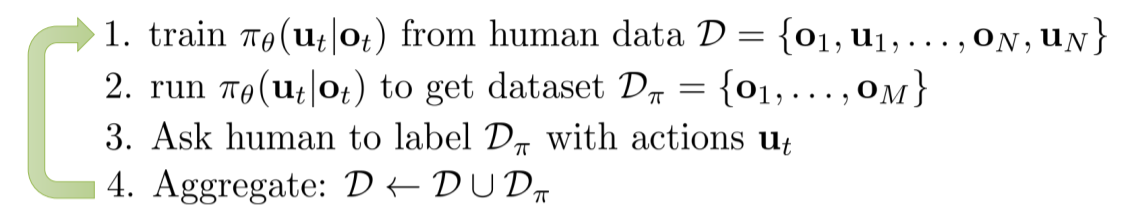
\includegraphics[width=0.7\linewidth]{images/dagger.png}
    \caption{Dataset Aggregation (DAgger) algorithm}
    \label{fig:dagger}
  \end{center}
\end{figure}

Here, they train the parameterized policy class (a mathematical representation) using the demonstration dataset $D$. When the learned policy is executed, we need not reach the same underlying states as that of demonstration and as a result we end up with different set of observations. These observations are again labeled by humans and are appended to out data-set $D$. This is repeated until all observations generated by following our policy are labeled. This methods was tested on a quadrotor which navigates around unknown forests. The problems in these knid of algorithms is the relabeling part. Humans do not know the exact action given a situation. We rely heavily on the feedback and a string of observation. This was handled in a ad-hoc method in the paper \cite{dagger}. 

In \cite{lstm}, they record a human using game controller to steer the end-effector of Baxter robot in a simulation environment. They take as input a string of observation or history and output the next action. The histories are passed to a recurrent CNN based network model. The following figure.\ref{fig:lstm} shows the 3 layer recurrent network of (Long short-term memory) LSTM\cite{lstmbirth}. The networks take as input the pose of the end effector $e$ anf the pose of the object $q$ and outputs parameters for a Gaussian mixture model. During task execution, they sample from this GMM to get the next pose of the end effector and solve inverse kinematics to execute the action. This method shows an example where imitation learning works out of the box. The execution of this method is shown in \url{https://www.youtube.com/watch?v=9vYlIG2ozaM}. 

\begin{figure}[H]
  \begin{center}
    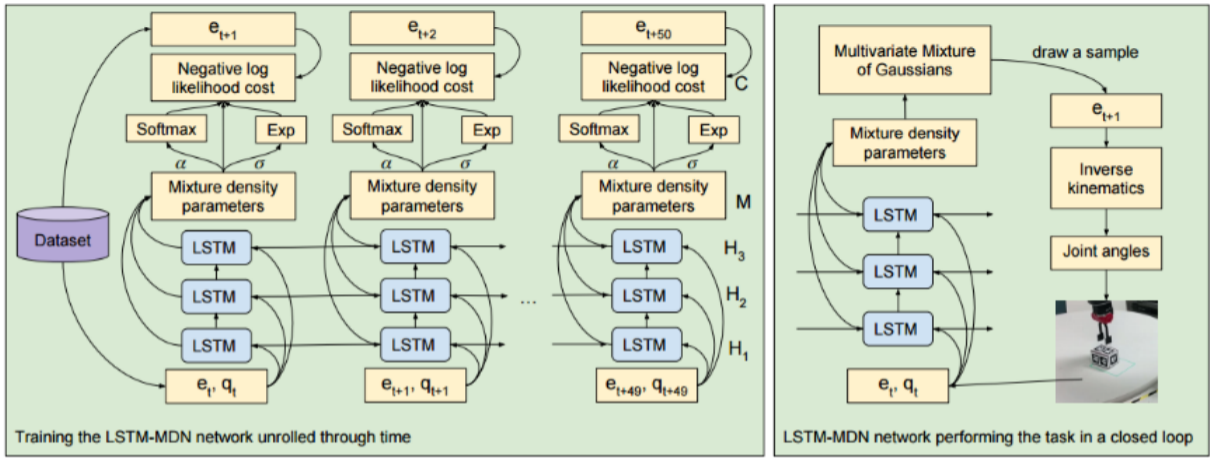
\includegraphics[width=\linewidth]{images/lstm.png}
    \caption{The LSTM network design for learning real manipulation tasks from virtual demonstrations.}
    \label{fig:lstm}
  \end{center}
\end{figure}


Generally imitation learning agents require task specific hacks. As a result, there exists significant literature that approach the problem differently - instead of mimicking the expert, one might want to discover the intent of the expert and thus perform tasks with the same intent. This motivates Inverse Reinforcement Learning (IRL) methods. We will survey different policy optimization methods, DRL, IRL and DRL using Policy Optimization. 


\subsection{Reinforcement Learning}

\begin{figure}[H]
  \begin{center}
    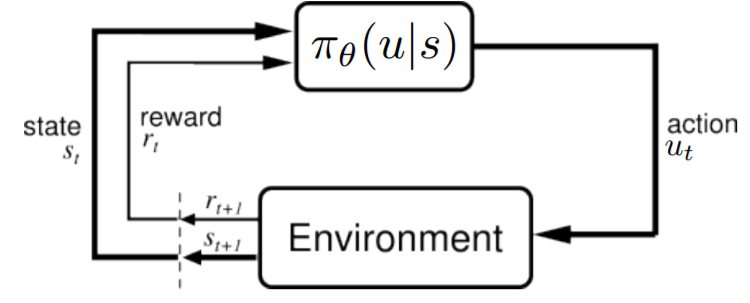
\includegraphics[width=0.7\linewidth]{images/rl.png}
    \caption{Reinforcement learning setting. \cite{drlnips}}
    \label{fig:rl}
  \end{center}
\end{figure}
A Markov Decision Process(MDP) is a tuple $(S,A,P,R,\gamma)$ where $S$ is the set of all states the agent can be in, $A$ is the set of all actions, $P : S \times A \times S \to [0,1]$ is the probability of landing in state $s'$ by taking action $a$ from state $s$, $R: S \to \mathbb{R}$ is the reward obtained for visiting state $s$, $\gamma \in [0,1)$ is the discount factor. A policy $\pi(u|s)$ is a probability distribution over actions given the current state. The aim of a reinforcement learning agent is to maximize the cumulative reward over policy 
\begin{align}
  \pi^* = \arg \max_\pi E[\sum_{t=0}^T \gamma^t R(s_t)|\pi]
\end{align}

	
Here the expectation is over the possible states we might land in following the same policy $\pi$ (even if $\pi$ is deterministic - due to stochastic dynamics) and the actions we might take given the state (in case of stochastic policy). The policy $\pi^*$ is said to be the optimal policy under the reward function $R$. 

The value of a state $s$ in an $MDP$ is defined as the maximum cumulative reward that one can acquire from that state

\begin{align}
  V(s) = \sum_s' P(s'|s,\pi(s)) (R(s') + \gamma V(s')) 
\end{align}

The Q-value of a state $s$ after committing to an action $a$ is given by

\begin{align}
  Q(s,a) = \sum_s' P(s'|s,a) (R(s') + \gamma V(s')) 
\end{align}

\subsection{Inverse Reinforcement Learning (IRL)}
In an IRL setup, we are given an $MDP \setminus R$ and an expert policy $\pi^*$. We assume that the expert's policy is optimal and try to come up with a reward function under which the optimal policy is $\pi^*$. In \cite{irl}, they use the following algorithm
\begin{enumerate}
\item Solve the forward control problem and find the optimal policy $\pi^o$ under the current reward function
\item Compare $\pi^o$ to $\pi^*$ 
\item Correct the reward function according to difference in $\pi^o$ and $\pi^*$ . If the difference is less than some $\epsilon$, terminate. Otherwise, go to step 1
\end{enumerate}

This was tested on a dynamic system - helicopter.\\ \textbf{Further study is required in this section}

\subsection{Policy Optimization}
The main motivation behind policy optimization is that it is often hard to define value function or Q function for a specific task. For example, in the task of grasping, one can easily accept a the set of actions (the policy) to be good. However, assigning a value to particular pose during the grasping problem is harder to track \cite{drlnips}. 


 In policy optimization, the way we parameterize the policy $\pi$ using $\theta$. For example, the parameters $\theta$ may be the weights in a huge neural networks that maps states to actions or directly observations to actions. The reinforcement learning objective in the context of policy optimization becomes, 
\begin{align}
  \theta = \arg \max_\theta E[\sum_{t=0}^TR(s_t)|\pi_\theta]
\end{align}
Often stochastic policy class is chosen to smooth out the policy optimization problem in case the underlying reward function is discontinuous. This works better even though we know that we only need a deterministic policy. 

\subsubsection{Cross Entropy Method}

This is a evolution (genetic algorithm) based method. The following shows the algorithm.  

\begin{figure}[H]
  \begin{center}
    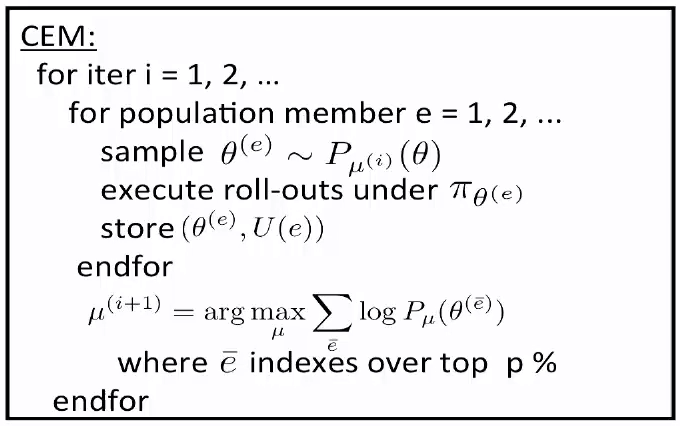
\includegraphics[width=0.7\linewidth]{images/cem.png}
    \caption{Algorithm - Cross Entropy Method}
    \label{fig:cem}
  \end{center}
\end{figure}
 
In the above algorithm we have a parameterized distribution $P_\mu$ for the parameter $\theta$ of the policy. We first sample $n$ parameters from $P_\mu$ that is $\theta^{(e)} \sim P_{\mu^{(i)}}(\theta)$. We execute roll-outs for each of the member in the population and find their cumulative reward $U(e)$. We pick the top $p\%$ individuals with respect to their $U$ of the population and perform a soft-max to update the parameter of our distribution. 

There are several different ways one could update the parameter $\mu$. In \cite{rwr} they perform a reward weighted regression in which the parameter update is given by 

\begin{align}
\mu^{(i+1)} = \arg \max_{\mu} \sum_eq(U(e),P_\mu(\theta^{(e)}))\log{P_\mu(\theta^{(e)}}) 
\end{align}
Here each individual is weighted by a function $q$ of the utility if that individual $U(e)$ and the probability of sampling the parameter $\theta^{(e)}$ from distribution $P_\mu$. In \cite{pi}, instead of picking top $p\%$, you look at all roll-outs and you weigh each roll out by exponentiated utility value $U(e)$ of that roll-out. The update is given by,

\begin{align}
\mu^{(i+1)} = \arg \max_{\mu} \sum_e \exp(\lambda U(e)) \log{P_\mu(\theta^{(e)})}
\end{align}

In \cite{cmaes}, we keep a distribution in a form of a Gaussian  parameterized by mean $\mu$ and covariance $\Sigma$. The update here is given by,
\begin{align}
(\mu^{(i+1)}, \Sigma^{(i+1)}) = \arg \max_{\mu,\Sigma }w(U(\bar{e}))\log{\mathcal{N}(\theta^{(\bar{e}};\mu,\Sigma)}
\end{align}

In \cite{power}, we optimize the expected log probabilities of the roll-outs that we got. The distributions are again assumed to be Gaussian The update here is,
\begin{align}
\mu^{(i+1)} = \mu^{(i)} + \Big(\sum_e(\theta^{(e)}-\mu^{(i)})U(e)\Big)/ \Big( \sum_e U(e) \Big)
\end{align}

This method, called PoWER, has been tested on a rather dynamic task where the robot arm has to swing a ball and drop in a cup it is holding. The link here shows the demonstration of PoWER in action - \url{https://www.youtube.com/watch?v=qtqubguikMk}

The main problem with these methods is that, they work well in case we need to find relatively few parameters. In case we want to learn the parameters of a neural net with hundred thousand parameters, it is difficult to make these methods work. 

Another way to approach this would be to use policy gradient methods. This is where the stochastic policy smooths out a discontinuous reward function. The gaol here can be broadly described as 

\begin{align}
\max_{\theta}U(\theta) = \max_{\theta }\sum_{\tau{}}P(\tau{} ;\theta)R(\tau{})
\end{align}
The gradient is given by 
\begin{align}
\bigtriangledown_\theta U(\theta) = \sum_\tau P(\tau;\theta) \bigtriangledown_\theta \log{P(\tau;\theta)} R(\tau)
\end{align}
Empirically, this is estimated in \cite{gpomdp} as,
\begin{align}
\bigtriangledown_\theta U(\theta) = \frac{1}{m}\sum_{i=1}^m \bigtriangledown_\theta \log{P(\tau;\theta)} R(\tau)
\end{align}
Intuitively, this just moves the parameters in the direction in which the probability of paths with positive R is increased and that of negative R is decreased.  

In a Markovian process, the gradient of the probability $P$ of a path $\tau$ becomes independent of the system dynamics. That is,
\begin{align*}
 \bigtriangledown_\theta \log{P(\tau;\theta)} &=  \bigtriangledown_\theta \log \Big[ \Pi_{t=0}^H P(\cdot)  \pi_{\theta}(\cdot) \Big]\\
 &= \sum_{t=0}^H \bigtriangledown_\theta \log{\pi_\theta(u_t^{(i)}|s_t^{(i)})}
\end{align*}

The bias of the method is proved to be zero and several variance reduction techniques are discussed in \cite{var} for the empirical estimate of the gradient.

In \cite{approx}, they come up with a method that optimizes an approximation to objective function (cumulative reward), a surrogate objective, which makes sure that we monotonically increase the reward while using gradient method. Also, \cite{trpo} guarantees monotonic increase in reward for highly non linear parametric policy such as the ones in neural nets. This allows us to use deep networks for the policy and still apply policy gradient methods. This allows us to effectively combine deep learning and robotics unlike imitation learning.

\section{Conclusion}
The report summarizes some deep learning methods for imitation learning and policy optimization methods. Need to read more on inverse reinforcement learning and form a "Big picture" of how to approach Learning from Demonstration problems.  

\begin{thebibliography}{8}
\bibitem{cmaes}
Hansen, Nikolaus, and Andreas Ostermeier. "Adapting arbitrary normal mutation distributions in evolution strategies: The covariance matrix adaptation." Evolutionary Computation, 1996., Proceedings of IEEE International Conference on. IEEE, 1996.
\bibitem{lstmbirth}
Hochreiter, Sepp, and Jürgen Schmidhuber. "Long short-term memory." Neural computation 9.8 (1997): 1735-1780.
\bibitem{rwr}
Dayan, Peter, and Geoffrey E. Hinton. "Using expectation-maximization for reinforcement learning." Neural Computation 9.2 (1997): 271-278.
\bibitem{gpomdp}
Baxter, Jonathan, and Peter L. Bartlett. "Infinite-horizon policy-gradient estimation." Journal of Artificial Intelligence Research 15 (2001): 319-350.
\bibitem{approx}
Kakade, Sham, and John Langford. "Approximately optimal approximate reinforcement learning." ICML. Vol. 2. 2002.
\bibitem{var}
Greensmith, Evan, Peter L. Bartlett, and Jonathan Baxter. "Variance reduction techniques for gradient estimates in reinforcement learning." Journal of Machine Learning Research 5.Nov (2004): 1471-1530.
\bibitem{irl}
Abbeel, Pieter, and Andrew Y. Ng. "Apprenticeship learning via inverse reinforcement learning." Proceedings of the twenty-first international conference on Machine learning. ACM, 2004.
\bibitem{power}
Kober, Jens, and Jan R. Peters. "Policy search for motor primitives in robotics." Advances in neural information processing systems. 2009.
\bibitem{pi}
Theodorou, Evangelos, Jonas Buchli, and Stefan Schaal. "A generalized path integral control approach to reinforcement learning." Journal of Machine Learning Research 11.Nov (2010): 3137-3181.
\bibitem{dagger}
Ross, Stéphane, Geoffrey J. Gordon, and Drew Bagnell. "A Reduction of Imitation Learning and Structured Prediction to No-Regret Online Learning." AISTATS. Vol. 1. No. 2. 2011.
\bibitem{trpo}
Schulman, John, et al. "Trust Region Policy Optimization." ICML. 2015.
\bibitem{nvidia}
Bojarski, Mariusz, et al. "End to end learning for self-driving cars." arXiv preprint arXiv:1604.07316 (2016).
\bibitem{lstm}
Rahmatizadeh, Rouhollah, et al. "Learning real manipulation tasks from virtual demonstrations using LSTM." arXiv preprint arXiv:1603.03833 (2016).
\bibitem{drlnips}
Shulman, Abbeel. Deep Reinforcement Learning Through Policy Optimization. NIPS 2016. https://goo.gl/TACjs6
\bibitem{walking}
\url{https://www.youtube.com/watch?v=kl_G95uKTHw&t=1305s}
\end{thebibliography}
\end{document}

